%File: formatting-instruction.tex
\documentclass[letterpaper]{article}
\usepackage{xcolor}
\usepackage{graphicx}

\usepackage{flairs}%aaai

\usepackage{times}
\usepackage{helvet}
\usepackage{courier}
\frenchspacing
\setlength{\pdfpagewidth}{8.5in}
\setlength{\pdfpageheight}{11in}

\pdfinfo{
/Title (Evaluating Neuro-Symbolic Reinforcement Learning in Maritime Capture-the-Flag)
/Author (Yahya Masri, Akshith Ambekar, Tuga Wangjie, Armin Khazai, Zawadul Haque, Prithviraj Dasgupta)
/Keywords (Neuro-Symbolic AI, Reinforcement Learning, Multi-Agent Systems, Maritime Capture-the-Flag, Linear Temporal Logic, PyQuaticus)
}

% Keep section numbering off to match the FLAIRS tutorial-style appearance.
\setcounter{secnumdepth}{0}

\begin{document}

\title{Evaluating Neuro-Symbolic Reinforcement Learning in Maritime Capture-the-Flag}

\author{Yahya Masri, Akshith Ambekar, \\
Armin Khazai, Tuga Wangjie, Zawadul Haque\\
Department of Computer Science\\
George Mason University\\
Fairfax, VA, USA
\And Prithviraj Dasgupta\\
Distributed Intelligent Systems Section\\
Information Technology Division\\
U. S. Naval Research Laboratory, Washington, DC, USA
}

\maketitle

\begin{abstract}
\begin{quote}
Reinforcement learning (RL) provides a promising approach for learning autonomous behaviors in competitive multi-agent environments, but policies learned solely through reward optimization can be difficult to constrain using explicit mission rules and behavioral requirements. In this work, we investigate neuro-symbolic guidance for reinforcement learning agents in Maritime Capture-the-Flag using PyQuaticus. Our system translates natural-language mission requirements into finite-trace Linear Temporal Logic specifications, validates them, and uses temporal-state information and reward shaping to guide Proximal Policy Optimization policies. We also evaluate a bounds-only action shield in a matched 3-vs-3 ablation. In a five-seed 1-vs-1 patrol study, softened neuro-symbolic guidance with no reward penalty for tagging achieved 138 captures in 150 held-out episodes. The promoted policies achieved no flag pickups or captures in 150 episodes against a chasing defender, despite entering opponent territory in every episode. Additional two-seed recovery experiments did not restore flag acquisition. These results show that guidance effects depend on reward design and opponent behavior: strong performance against patrol did not transfer to active pursuit. For the evaluated policy, the primary failure occurred between entering enemy territory and acquiring the flag.
\end{quote}
\end{abstract}

\section{Introduction}

Reinforcement learning (RL) provides a general framework for learning sequential decision-making policies from interaction with an environment. In multi-agent settings, the problem becomes more difficult because an agent must reason not only about the environment and its own objective, but also about teammates and opponents whose behavior may alter the consequences of an action. Competitive games are therefore useful experimental domains for studying autonomous decision making under interaction, uncertainty, and strategic opposition.

Maritime Capture-the-Flag (MCTF) provides one such domain. An autonomous agent must navigate a bounded environment, cross into opposing territory, acquire an opponent's flag, return to friendly territory, and complete a capture while responding to defenders. In team settings, agents must additionally coordinate offensive and defensive behavior. The task is simple enough to define precisely, but rich enough to expose problems in exploration, reward design, coordination, and robustness to opponent behavior.

A recurring difficulty in RL is that a reward function does not necessarily provide a complete specification of desired behavior. A policy may improve its expected return while violating rules, ignoring intermediate mission requirements, or exploiting tradeoffs that differ from the intent of a human designer. This motivates methods that combine learned policies with explicit symbolic representations of desired behavior.

In this work, we investigate a neuro-symbolic approach in which natural-language mission requirements are translated into finite-trace Linear Temporal Logic (LTLf) formulas and incorporated into RL through several forms of guidance. The symbolic component is used to represent temporal mission structure, while the learned policy remains responsible for selecting actions in the environment. The language model is therefore outside the gameplay loop: it is used to construct a formal mission specification before training or evaluation rather than to choose actions at every time step.

The main research question considered in this paper is:

\begin{quote}
\textit{How do temporal-logic-based neuro-symbolic guidance mechanisms affect task completion and constraint-related behavior in MCTF, and how does their effectiveness change as opponent behavior becomes more adversarial?}
\end{quote}

A second question concerns where task execution fails when an agent does not complete a capture. Capture-the-Flag can be decomposed into a sequence of observable stages: entering opponent territory, approaching the flag, acquiring the flag, returning across the midfield boundary, and completing the capture. Evaluating only final capture rate can hide important differences between policies that fail at different stages.

To study these questions, we developed an end-to-end system that connects English-to-LTLf translation, formula validation and grounding, temporal monitoring, temporal-state features, reward shaping, shielding, PPO-based learning, PyQuaticus execution, trajectory recording, and held-out evaluation. We first perform a matched 3-vs-3 ablation comparing a neural baseline with temporal-state guidance, reward shaping, shielding, and combined guidance. We then conduct a staged 1-vs-1 study against scripted patrol and chase opponents. Finally, we perform a focused diagnostic study to determine whether additional approach and evasion shaping can recover flag acquisition against the chasing defender.

The results show that the effect of guidance is highly conditional on both the objective design and the opponent. In the frozen 3-vs-3 study, full guidance produced low tag and measured rule-violation rates and the highest mean fixed common task reward among the evaluated methods, but it did not complete a capture. In the later 1-vs-1 study, softened guidance without a training penalty for tagging achieved 138 captures in 150 patrol episodes across five training seeds. When the same promoted policy was evaluated against a chasing defender, it entered enemy territory in all 150 held-out episodes but acquired the flag in none of them. These results suggest that constraint-related behavior and task completion should be evaluated separately, and that increasingly adversarial opponent behavior can expose failure modes that are not visible in easier environments.

The principal contributions of this work are: (1) an end-to-end pipeline for representing natural-language mission requirements as LTLf and incorporating them into PPO-based control; (2) a controlled ablation of temporal-state, reward-shaping, shielding, and combined guidance in team Capture-the-Flag; (3) a staged evaluation that identifies a transition from high patrol performance to complete failure before flag acquisition against an active chaser; and (4) a controlled benchmark of our CTF-focused English-to-LTLf translator against a translation-only adapter based on the existing LTLCodeGen project.

\section{Related Work}

\subsection{Adversarial Multi-Agent Learning and Maritime Capture-the-Flag}

Adversarial games provide a controlled setting in which learned agents must respond not only to an environment but also to other decision makers whose behavior can directly oppose their objectives. This perspective has been used repeatedly in work associated with the U.S. Naval Research Laboratory. Dasgupta and Kliem study deep RL in the asymmetric real-time strategy game Hunting-of-the-Plark and investigate self-play and strategy diversity as mechanisms for improving behavior beyond an equilibrium-like outcome \cite{dasgupta2023strategy}. More recently, Rajbhandari, Dasgupta, and Sofge use MCTF as an evaluation domain for BERTeam, a transformer-based team-selection method integrated with coevolutionary deep RL \cite{rajbhandari2025transformer}. NRL-affiliated work has also examined multi-agent RL in the CAGE autonomous cyber-defense challenge, illustrating the broader use of adversarial environments to study scalable multi-agent learning \cite{kiely2025cage}. These studies motivate treating Capture-the-Flag not merely as a game, but as a compact testbed for coordination, adaptation, and strategic interaction.

The work most directly related to our domain is the MCTF study of Beason et al. \cite{beason2024mctf}. Their experiments evaluate behavior-based and deep-RL autonomy on teams of unmanned surface vehicles using the Aquaticus test bed, with Pyquaticus used as a lightweight environment for training RL agents. In the reported competition, the implemented behavior-based cooperative agents outperformed the deep-RL agents. Importantly for the present work, the authors identify reward shaping, improved simulation-to-real integration, and extending rule-based cooperation to respond to safety and security events according to human intent as future research directions. Our work follows a complementary direction: rather than improving team selection or behavior trees, we investigate whether explicit temporal mission structure can guide a learned policy and how that guidance behaves as the opponent becomes more adversarial.

\subsection{Temporal-Logic-Guided Reinforcement Learning}

A central difficulty in RL is specifying complex objectives through scalar rewards. Alur et al. survey specification-guided RL and note that manually encoding temporally structured objectives as low-level state-based rewards can be difficult and that alternative reward encodings can substantially affect learning \cite{alur2026specification}. Formal specification languages such as Linear Temporal Logic (LTL) provide a precise representation of ordering, persistence, and eventuality that can be used alongside learning rather than replacing it.

Several approaches use temporal logic to expose task structure to a learned controller. León, Shanahan, and Belardinelli introduce a neuro-symbolic architecture in which a symbolic temporal-logic component transforms task specifications into a representation used by a deep-RL agent, with an emphasis on systematic generalization to unseen instructions \cite{leon2020systematic}. Jiang et al. derive reward-shaping functions from temporal-logic domain knowledge, demonstrating that a formal specification can provide intermediate learning signals without changing the underlying task objective \cite{jiang2021temporal}. These approaches motivate two of the mechanisms studied here: temporal-state information and temporal-logic-based reward shaping.

Shielding provides a stronger form of symbolic intervention. Prior work synthesizes reactive shields from temporal-logic safety specifications to monitor and correct actions that would violate those specifications \cite{alshiekh2018shielding}. Any shield guarantee is limited by the world model and specification used to construct it \cite{konighofer2025shields}.

Related maritime work also demonstrates the growing use of neuro-symbolic architectures for autonomous surface vehicles. Huang et al. propose NSC-Marine, which combines semantic reasoning, LLM-based rule interpretation, deterministic safety-bounded execution, energy-aware planning, and fault reconfiguration for multi-USV coordination \cite{huang2026nscmarine}. Their evaluation is simulation-only and uses a substantially different controller architecture and task from ours, but it provides a useful example of separating symbolic rule reasoning from low-level execution in a maritime setting. More broadly, Rodrigues et al. combine LLM-based semantic retrieval, formal constraints, digital-twin modeling, and game-theoretic multi-agent learning for industrial process control \cite{rodrigues2026agentic}. Together, these systems illustrate a broader trend toward hybrid architectures in which symbolic or semantic reasoning structures the problem presented to a learned or optimized controller.

\subsection{Natural Language to Temporal Logic}

A separate line of research concerns constructing formal temporal specifications from natural language. Wang et al. learn an executable semantic parser that maps natural-language commands to latent LTL representations using execution examples and a planner, demonstrating that language-to-LTL grounding can be treated as an executable semantic parsing problem \cite{wang2021semantic}. Hsiung et al. introduce lifted LTL and an intermediate contextual representation to improve generalization to unseen object references and domains \cite{hsiung2022lifted}. These approaches predate current large-language-model pipelines but establish grounding and semantic generalization as central challenges.

Recent work increasingly uses large language models (LLMs) to reduce annotation requirements and improve flexibility. Pan, Chou, and Berenson generate synthetic LTL-language data and use constrained decoding to improve syntactic validity while learning from limited human annotation \cite{pan2023dataefficient}. Lang2LTL uses a modular LLM-based pipeline to ground complex temporal navigation commands into LTL specifications in previously unseen environments \cite{liu2023lang2ltl}. LTLCodeGen takes a different approach by asking an LLM to generate code that produces syntactically correct LTL, then connects the resulting formula to semantic mapping and motion planning \cite{rabiei2025ltlcodegen}. These methods highlight an important distinction for our translator evaluation: syntactic validity and compilation are necessary, but they do not by themselves establish that a generated formula preserves the intended task semantics.

The present work lies at the intersection of these research threads. Prior studies have separately examined RL for MCTF, temporal-logic-guided RL, shielding and reward shaping, and natural-language translation to temporal logic. Our study instead evaluates an end-to-end pipeline in which natural-language mission intent is translated to finite-trace temporal logic and then incorporated into PPO through multiple forms of guidance. We focus specifically on how these guidance mechanisms affect task completion and constraint-related behavior as opponent behavior becomes more adversarial, and on identifying the stage of the Capture-the-Flag objective at which learned behavior fails.

\section{Methodology}

\subsection{System Overview}

The system is organized as a pipeline from mission specification to policy evaluation. A natural-language mission statement is first translated into an LTLf formula. The generated formula is then parsed, grounded against the predicates available in the Capture-the-Flag environment, and checked for validity before it is used by the learning system. During training and evaluation, the symbolic specification can influence the policy through temporal-state information, reward shaping, or an action shield. PPO remains responsible for choosing among the available discrete waypoint actions.

\begin{figure}[htbp]
\centering
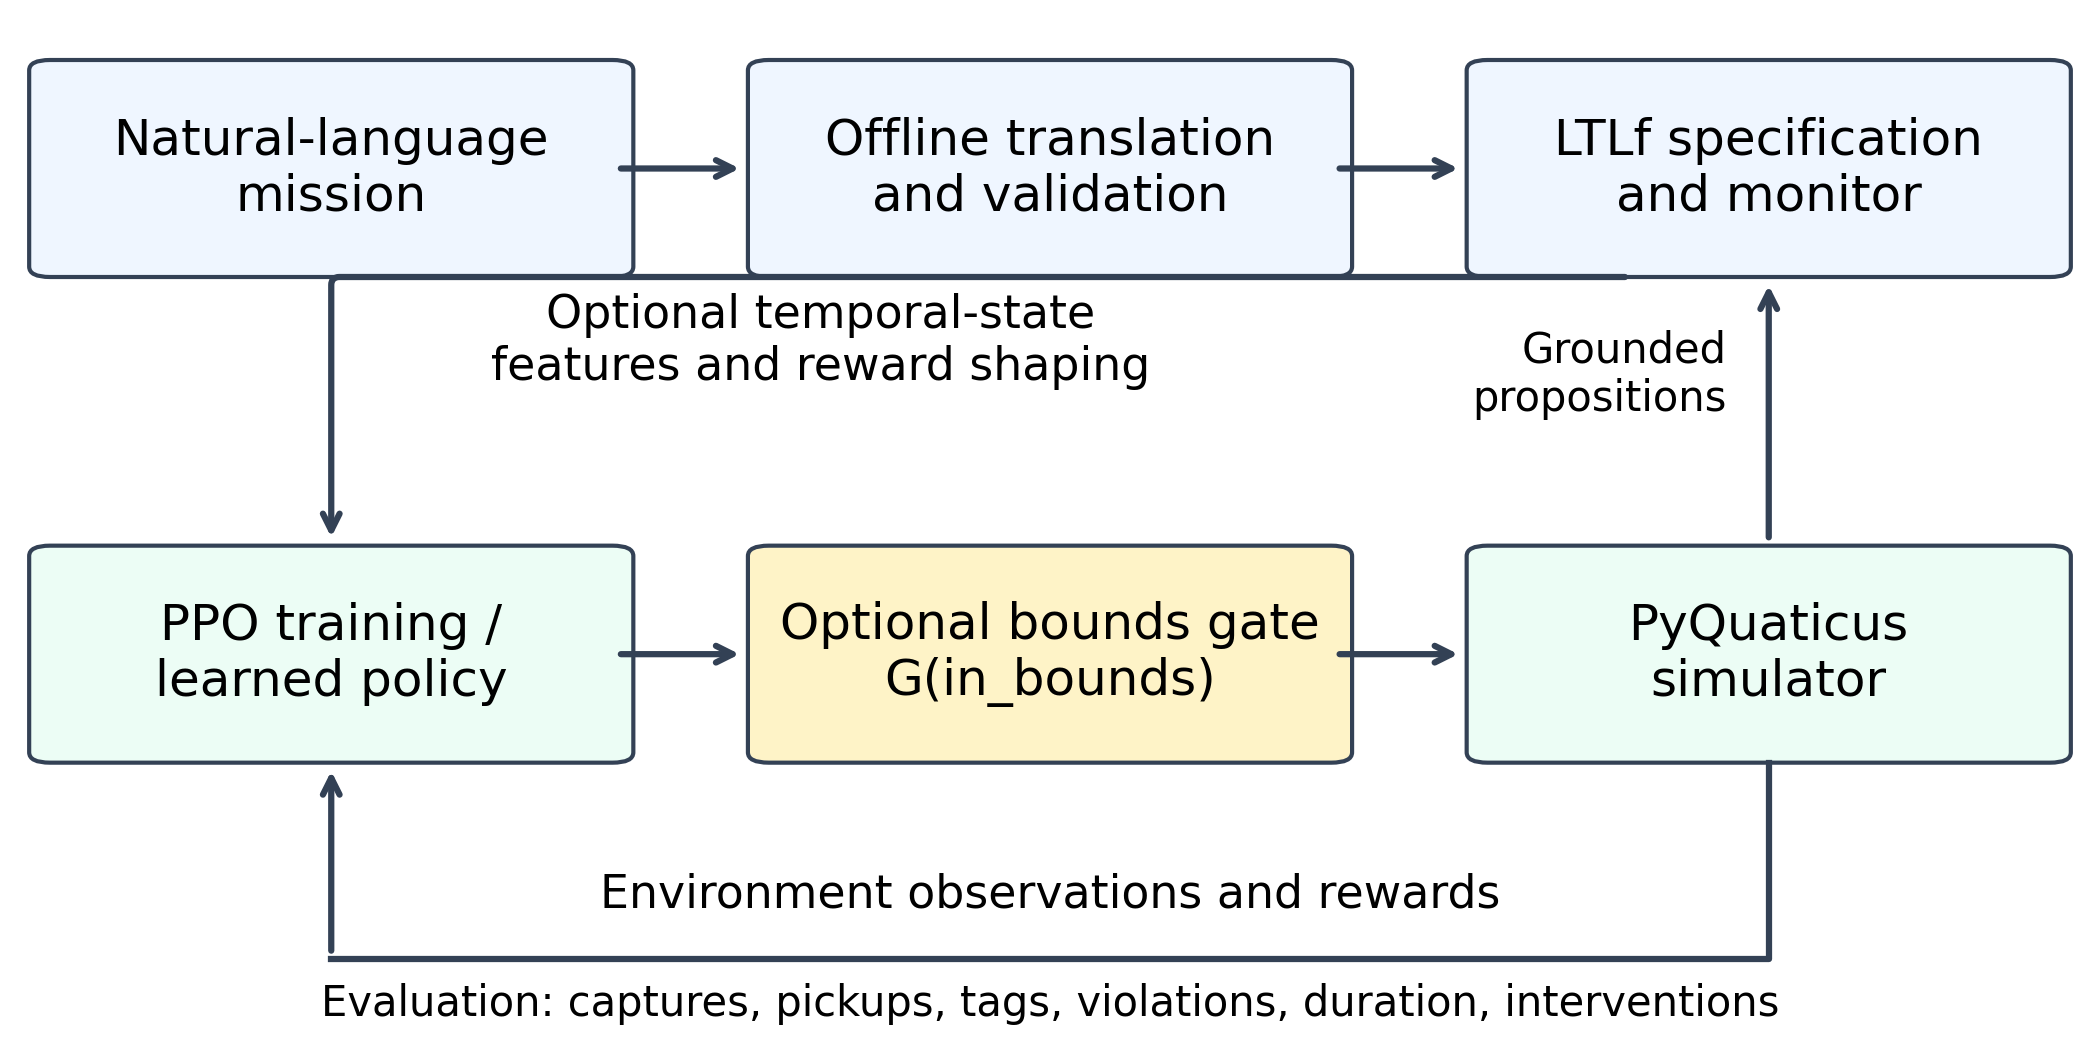
\includegraphics[width=\columnwidth]{figures/figure1_system_architecture.png}
\caption{Implemented neuro-symbolic pipeline. Offline translation and validation produce an LTLf mission monitor; optional temporal features and shaping influence PPO training. A separate optional bounds gate filters proposed actions. The runtime-only study evaluates the same saved policy with this gate disabled and enabled.}
\label{fig:system-architecture}
\end{figure}

The original implementation used Python 3.10, Stable-Baselines3 PPO, and pinned PyQuaticus Heron dynamics. Policies select among eight discrete waypoint-style action primitives. Each selected primitive is applied for a short decision interval; the learned policy therefore chooses among higher-level movement primitives rather than directly controlling low-level vessel dynamics.

\subsection{Original Proposal and Implemented Guidance}

The original project proposal was to train a neural policy without symbolic guidance and apply a temporal-logic action shield during deployment. The implemented research framework subsequently expanded this design to include temporal-state features in the policy observation and reward shaping during training, with action shielding enabled in selected experimental conditions. These are distinct interventions: observation augmentation and shaping affect the learned policy, whereas a deployment-only shield filters the actions of an already trained policy.

In particular, the frozen 3-vs-3 shield-only condition enabled the bounds gate during both training and evaluation. Its results therefore do not isolate the effect of adding a runtime shield to an unchanged neural checkpoint. We evaluate that narrower question separately using paired shield-off and shield-on evaluations of the same saved neural policies.

The language model is invoked before gameplay to construct the specification. Per-step temporal monitoring uses the compiled finite-state monitor and does not require a language-model request. The computational cost of monitoring must therefore be distinguished from the cost of language-model translation and from simulator prediction within the shield.

\subsection{Temporal Mission Specification}

The central mission used in the later staged experiments was represented as

\[
G(\mathrm{InBounds}) \land
F(\mathrm{HasFlag} \land F(\mathrm{Captured}))
\]

where $\mathrm{InBounds}$, $\mathrm{HasFlag}$, and $\mathrm{Captured}$
correspond to the implementation predicates
\verb|in_bounds|, \verb|has_flag|, and \verb|captured|,
respectively.

The first term requires the agent to remain in bounds throughout the finite trace. The second term represents an ordered mission objective: at some point the agent must possess the flag, and after that point a capture must eventually occur. Earlier specifications included harder safety and role constraints. During the project, provenance review separated translated mission intent from human-added role and safety rules, and the ordered flag-acquisition objective was restored explicitly.

The project used three principal mechanisms for incorporating symbolic information into learning. Temporal-state guidance augments the policy observation with information derived from the progress of the temporal monitor. Reward shaping adds intermediate rewards or penalties associated with progress toward or away from temporal objectives. Shielding can reject or redirect actions judged to violate specified constraints. In the frozen matched 3-vs-3 experiment, the hard shield enforced arena bounds only; tagging and the designated defender's centerline position were monitored as rule violations, not enforced by the shield. Thus, ``shield-only'' refers to bounds shielding and does not mean the shield hard-enforced the full LTL role and safety contract. A combined condition applies multiple mechanisms simultaneously. The implemented gate tests a bounded set of one-step simulator successors and commits a candidate whose bounds-monitor state remains live. If every tested candidate is rejected, the episode terminates without advancing the simulator. Such a deadlock does not prove that no safe action exists, because the candidate set is not exhaustive. This local-model check does not guarantee collision avoidance, absence of tagging, eventual flag capture, or satisfaction of the complete mission specification.
    
\subsection{Earlier Single-Seed Exploratory Run}

Before the matched and staged studies, we ran an exploratory single-seed comparison with 24,576 training decisions. The guided policy captured the flag in 20/20 held-out episodes against a static opponent, 18/20 against a patrol opponent, and 0/20 against a chasing opponent. The neural baseline captured in 0/20 episodes against each opponent. These results came from an earlier configuration and one training seed; they are reported as project history and are not pooled with the later experiments or used as a multi-seed comparison.

\subsection{Frozen Matched 3-vs-3 Ablation}

The first main experiment was a matched five-method ablation in a 3-vs-3 team environment. The evaluated methods were: neural PPO, temporal state only, reward shaping only, shielding only, and full guidance. Each method used shared-policy PPO and was trained against the scripted chase opponent on the standard map with five training seeds.

Each training run requested 100,000 individual-agent transitions. PPO's rollout structure resulted in 100,608 transitions, corresponding to 33,536 joint team decisions. Each trained policy was evaluated on the same held-out episode seeds for each map and opponent condition. Across the full evaluation, the study contained 6,750 held-out episodes.

For comparison across methods, evaluation used a fixed common task reward of 20 per capture, 2 per pickup, minus 2 per tag event, and minus 0.01 per simulator step. Shaping rewards and shield abort penalties were excluded from this common metric so that methods could be compared using the same task-level measure.

\subsection{Staged 1-vs-1 Evaluation}

The second main study focused on offensive task completion in 1-vs-1 play. Four methods were evaluated against a scripted patrol defender: neural PPO, temporal state only, softened neuro-symbolic guidance with a tag penalty of 1.0, and softened neuro-symbolic guidance with a tag penalty of 0.0.

The softened guidance configuration used a capture reward of 25, pickup reward of 8, time penalty of 0.005, potential scale of 3, acceptance bonus of 8, and failure penalty of 0. The two softened conditions differed only in the learned task reward's tag penalty.

Each condition was trained with five seeds and evaluated over 30 held-out episodes per seed. Before running the more difficult chase stage, we used a pre-defined promotion rule: at least three of five seeds had to reach a 10\% capture rate, and the pooled capture rate across the 150 held-out episodes had to be at least 10\%. Only the softened condition with zero training penalty for tagging passed this screen and advanced to chase evaluation.

The promoted policy was then evaluated against a scripted chasing defender using the same five-seed structure and 30 held-out episodes per seed. In addition to final capture rate, we recorded intermediate task stages including whether the agent reached enemy territory and whether it acquired the flag. This allowed failure to be localized within the offensive task sequence.

\subsection{Chase-Recovery Diagnostic}

After the promoted policy failed to acquire the flag against chase, we performed an exploratory diagnostic to test whether additional pre-pickup guidance could improve approach behavior. The diagnostic retained the promoted LTLf mission, PPO configuration, and action abstraction, while disabling the shield.

Three variants were evaluated: the current no-tag-penalty baseline, dense flag-progress shaping, and a combined flag-progress plus evasion condition with an additional distance feature. The diagnostic used two training seeds and 20 evaluation episodes per seed for each condition. Because of this smaller design, it was treated as a screening experiment rather than a confirmatory comparison.

The diagnostic measured captures, pickups, minimum distance to the enemy flag, tags before pickup, time spent in enemy territory, and minimum distance to the defender. A pre-defined screen required at least a 10\% pickup rate and at least a 10\% improvement in mean minimum flag distance relative to the baseline before a candidate would be considered for further confirmation.

\subsection{Paired Runtime-Shield-Only Evaluation}

We conducted a separate exploratory evaluation using two neural policies from the completed 1-vs-1 patrol study. Both checkpoints had been trained without reward shaping, temporal-state input, or shielding. Each unchanged checkpoint was evaluated deterministically with the existing bounds gate disabled and enabled, using identical held-out episode seeds, observations, action primitives, opponent settings, and horizons. The evaluation covered standard, wide, and narrow maps against static, patrol, and chase opponents, with ten held-out episodes per map--opponent combination and training seed: 180 episodes per arm and 360 episodes in total. No additional policy training was performed.

We recorded captures, pickups, common task reward, tags, bounds violations, monitored mission satisfaction, successful capture times, episode duration, numerical terminations, and shield deadlocks. Additional event logs recorded proposed and substituted controls and intervention context before the successor was committed, including enemy-territory position, proximity to the enemy flag, and flag possession. Early deadlocks shorten exposure to time penalties and tagging, so common reward is interpreted together with duration and termination outcomes. The study has two independent training seeds and is treated as exploratory rather than confirmatory.

\subsection{Translator Benchmark}

The natural-language translation component was evaluated independently from policy learning. The benchmark contained 40 Capture-the-Flag statements across nine categories and 20 paraphrase pairs. Each method received three independent trials per statement, producing 120 measured outputs per method.

The comparison used the same OpenRouter model identifier, \texttt{nvidia/nemotron-3-ultra-550b-a55b:free}, and the same finite-trace validator and scorer for both translation methods. The first method was the project's current English-to-LTLf pipeline. The second was a translation-only adapter based on the existing LTLCodeGen project. It reused selected upstream translation components, including the few-shot prompt structure and logical operators, and adapted them to the CTF vocabulary and benchmark interface. Its outputs were interpreted through a restricted Python AST subset and passed through the same validator and scorer as our translator. This was not a full integration or reproduction of LTLCodeGen's robotics system.

Metrics included syntax validity, successful compilation, semantic correctness against project-authored reference formulas, unsupported predicates, repair rate, mean latency, and paraphrase equivalence. The reference formulas had not yet received independent human approval, so semantic-correctness results should be interpreted as agreement with the project's reference interpretation rather than as a universal measure of language understanding.

\section{Results}

\subsection{Frozen 3-vs-3 Ablation}

Table~\ref{tab:frozen} summarizes the main results of the frozen matched ablation. Captures were rare across all methods. The neural baseline completed 1 capture in 1,350 evaluation episodes, temporal-state guidance completed 3, and reward shaping, shielding, and full guidance completed none. All four observed captures occurred against static opponents; no method completed a capture against patrol or chase.

Despite the absence of captures, the full-guidance condition produced the highest mean fixed common task reward, $-2.383$, compared with $-2.650$ for neural PPO, $-2.600$ for temporal-state guidance, $-2.659$ for reward shaping, and $-2.720$ for shielding. Full guidance also had the lowest measured episode-level tag incidence, 0.37\%, and the lowest mean measured rule-violation steps, 0.699. Shield deadlocks occurred in 2.30\% of shield-only episodes and 2.81\% of full-guidance episodes. This result does not establish an overall performance advantage because the same policy completed no captures. Instead, it illustrates that constraint-related measurements and task completion can move in different directions.

\begin{table}[htbp]
\centering
\small
\setlength{\tabcolsep}{4pt}
\begin{tabular}{lrrr}
\hline
Method & Captures & Mean Reward & Tag Episodes \\
\hline
Neural & 1/1350 & -2.650 & 2.81\% \\
Temporal state & 3/1350 & -2.600 & 4.30\% \\
Reward shaping & 0/1350 & -2.659 & 8.15\% \\
Shield & 0/1350 & -2.720 & 13.11\% \\
Full guidance & 0/1350 & -2.383 & 0.37\% \\
\hline
\end{tabular}
\caption{Frozen matched 3-vs-3 ablation. Mean reward is the fixed common task reward used for cross-method evaluation.}
\label{tab:frozen}
\end{table}

\subsection{Patrol Evaluation}

The staged patrol study produced a substantially different outcome. Neural PPO completed 0 of 150 held-out episodes. Temporal-state-only guidance also completed 0 of 150, although it picked up the flag in 60 episodes. Softened guidance with a tag penalty of 1.0 completed 29 of 150 episodes, corresponding to a 19.3\% capture rate.

The strongest result was obtained after removing the training penalty for tagging while retaining the softened temporal mission and reward structure. This condition completed 138 of 150 held-out patrol episodes, corresponding to a 92.0\% pooled capture rate, and picked up the flag in 149 of 150 episodes. Per-seed capture counts were 24/30, 29/30, 30/30, 26/30, and 29/30. The result satisfied the pre-defined promotion criterion and was therefore advanced to the chase stage.

The improvement came with a change in constraint-related behavior. The zero-tag-penalty condition had tags in approximately 10.0\% of patrol evaluation episodes and measured violations in approximately 8.7\%, whereas the tag-penalty-1 condition had tag and violation episodes near 1.3\%. Thus the modification that substantially improved offensive task completion also relaxed behavior that had previously discouraged contact with the defender.

\begin{table}[htbp]
\centering
\small
\begin{tabular}{lrr}
\hline
Method & Captures & Pickups \\
\hline
Neural & 0/150 & 30/150 \\
Temporal state & 0/150 & 60/150 \\
Soft guidance, tag penalty 1 & 29/150 & 29/150 \\
Soft guidance, tag penalty 0 & 138/150 & 149/150 \\
\hline
\end{tabular}
\caption{Held-out 1-vs-1 patrol evaluation across five training seeds.}
\label{tab:patrol}
\end{table}

\subsection{Chase Evaluation}

The promoted zero-tag-penalty policy did not transfer to the chase opponent. Across five seeds and 150 held-out episodes, it completed zero captures and zero flag pickups. However, it entered enemy territory in all 150 episodes.

This distinction localizes the failure. The policy consistently completed the first stage of the offensive task by crossing midfield, but failed before flag acquisition. Mean tags received were approximately 2.46 per episode and approximately 87.3\% of episodes contained at least one measured violation. The result therefore cannot be described as a general failure to move offensively; instead, active pursuit disrupted the transition from entering opponent territory to acquiring the flag.

\subsection{Chase-Recovery Diagnostic}

None of the three diagnostic variants recovered flag acquisition. The current no-tag-penalty baseline, dense flag-progress shaping, and the combined flag-progress-plus-evasion condition each produced 0 pickups and 0 captures in 40 held-out episodes.

The baseline reached a mean minimum distance of 39.84 m from the enemy flag. Dense progress shaping increased this distance to 51.67 m, while the combined evasion and distance-feature condition increased it further to 67.98 m. At the same time, the combined evasion condition reduced tags before pickup to zero and increased separation from the defender. These measurements are consistent with a policy becoming more conservative with respect to the defender while making less progress toward the offensive objective.

Because the diagnostic used only two seeds per condition, this result should not be interpreted as a definitive causal comparison. It nevertheless shows that the tested recovery mechanisms did not satisfy the pre-defined promotion screen and suggests that simply increasing distance-based evasion incentives can conflict with flag-approach behavior.

\subsection{Runtime-Shield-Only Evaluation}

The paired runtime-only screen completed 360 episodes across two training seeds, three maps, and three opponents. Both arms produced zero captures and zero pickups in 180 episodes each. Neither neural checkpoint entered enemy territory, and neither arm recorded tags, bounds violations, numerical terminations, or shield deadlocks. Mean common task reward was $-2.400$ and mean episode duration was 240 simulator seconds in both arms. Monitored mission satisfaction was zero, and successful capture time was undefined because there were no captures.

The runtime gate performed 43,200 successor checks without substituting an action. All 180 matched pairs had identical recorded action and state trajectories. Thus, the shield was dormant in this sample: the policies failed to initiate offensive progress before any action filtering occurred. These observations establish neither a safety advantage nor suppression of offensive actions by deployment-only shielding. A meaningful intervention test requires a task-capable unshielded policy and states in which unsafe actions are actually proposed. With only two independent training seeds, this study is exploratory and does not support a superiority claim.

\begin{table}[htbp]
\centering
\small
\setlength{\tabcolsep}{3.5pt}
\begin{tabular}{lrr}
\hline
Metric & Shield off & Runtime shield \\
\hline
Episodes & 180 & 180 \\
Captures / pickups & 0 / 0 & 0 / 0 \\
Enemy-territory episodes & 0 & 0 \\
Tag / bounds-violation episodes & 0 / 0 & 0 / 0 \\
Deadlock episodes & 0 & 0 \\
Mean common task reward & -2.400 & -2.400 \\
Mean duration (seconds) & 240 & 240 \\
Shield substitutions & -- & 0 \\
\hline
\end{tabular}
\caption{Exploratory deployment-only comparison of the same two saved neural policies. The lack of unsafe proposals leaves intervention effects untested.}
\label{tab:runtime-shield}
\end{table}

\subsection{Translator Benchmark}

The current English-to-LTLf pipeline produced 93.75\% semantic correctness against the project-authored reference formulas, 98.96\% syntax validity, and 98.96\% compilation success across 120 measured outputs. Its mean latency was 34.9 s and its repair rate was 43.33\%.

The custom CTF-specific LTLCodeGen adapter produced 71.88\% semantic correctness, 100\% syntax validity, and 100\% compilation success. Its mean latency was 53.7 s and its repair rate was 15.00\%. Paraphrase-equivalence measurements were 84.0\% for the current pipeline and 80.77\% for the adapter over the pairs that could be compared.

These results favor the current pipeline on agreement with the project reference formulas, latency, and paraphrase consistency, while the adapter produced perfect syntax and compilation validity with fewer repairs. The comparison is specific to this dataset, model, prompt configuration, CTF adaptation, and finite-trace validator. It is not a comparison against the complete upstream LTLCodeGen robotics system.

\begin{table}[htbp]
\centering
\small
\begin{tabular}{lrr}
\hline
Metric & Current & CTF Adapter \\
\hline
Semantic correctness & 93.75\% & 71.88\% \\
Syntax valid & 98.96\% & 100\% \\
Compilable & 98.96\% & 100\% \\
Repair rate & 43.33\% & 15.00\% \\
Mean latency & 34.9 s & 53.7 s \\
\hline
\end{tabular}
\caption{English-to-LTLf translator benchmark. Each method produced 120 measured outputs using the same language model and validation pipeline.}
\label{tab:translator}
\end{table}

\section{Future Work}

The most immediate direction for future work is to address the failure to acquire the flag under active pursuit. The existing diagnostics indicate that simply increasing progress or evasion shaping is insufficient and can make the agent more conservative. A more targeted approach should inspect per-step reward contributions and state-action trajectories around the point at which the agent approaches the defender or the flag. This could support gated or directional evasion terms that activate only when they preserve progress toward the offensive objective.

A second direction is to expand the action representation. The present PPO policy selects from eight waypoint-style primitives. This abstraction is sufficient for successful capture in several static and patrol configurations, but it may limit maneuvering near an active defender. A richer action set or a hierarchical policy could provide more expressive local evasion while retaining higher-level symbolic mission guidance.

A third direction is to continue the staged curriculum beyond 1-vs-1 once a policy demonstrates reliable acquisition against chase. The current project includes shared-policy team-training infrastructure, but the confirmatory curriculum stopped before a successful learned 3-vs-3 stage because the promoted 1-vs-1 policy failed the chase criterion. Future experiments should therefore avoid claiming successful learned team coordination until a policy passes the more difficult offensive stages and advances through the curriculum.

The translation subsystem also requires further validation. The present benchmark uses project-authored reference formulas and should be followed by independent human review of those reference interpretations. Additional experiments could evaluate robustness to longer mission descriptions, compositional rules, conflicting requirements, and previously unseen predicates. A hybrid translator that combines the current pipeline's semantic performance with the adapter's syntax reliability and lower repair frequency is another possible direction.

Finally, future studies should treat training seeds as the independent experimental units and report uncertainty over seed-level outcomes. Larger multi-seed confirmatory studies would help determine whether the patrol result persists under new maps, different scripted defenders, altered dynamics, and changed training budgets. These extensions are necessary before drawing broader conclusions about the generality of neuro-symbolic guidance.

\section{Conclusion}

This work evaluated neuro-symbolic reinforcement learning in Maritime Capture-the-Flag using an end-to-end system that connects natural-language mission specification, LTLf validation and monitoring, symbolic guidance, PPO-based learning, and PyQuaticus execution. Rather than producing a single conclusion that neuro-symbolic guidance is uniformly better or worse than neural reinforcement learning, the experiments show that its effect depends strongly on both the form of guidance and the behavior of the opponent.

In the frozen 3-vs-3 ablation, combined guidance reduced measured tags and rule violations and produced the highest mean fixed common task reward, but it completed no captures. In the later staged 1-vs-1 study, softened guidance without a training penalty for tagging achieved 138 captures in 150 held-out patrol episodes across five seeds. The same promoted policies then achieved zero pickups and zero captures in 150 episodes against an active chasing defender, despite entering enemy territory in every episode. Additional diagnostic variants did not recover flag acquisition.

The separate runtime-only screen left the evaluated neural checkpoints unchanged because the bounds gate never intervened; it provides no evidence that deployment-only shielding recovers offensive behavior.

The main empirical conclusion is therefore not that neuro-symbolic guidance universally improves task performance, but that symbolic guidance can substantially alter the balance between constraint-related behavior and task execution. The patrol and chase results further show the importance of evaluating policies across increasing levels of adversarial difficulty and of measuring intermediate task stages rather than relying only on final reward or capture rate. For the system studied here, the dominant unresolved failure occurs between entering opponent territory and acquiring the flag under active pursuit. This failure provides a concrete target for future work on reward design, action abstraction, and adaptive symbolic guidance.

% Bibliography supplied in CS491_references.bib and copied to references.bib.
\bibliographystyle{flairs}
\bibliography{references}

\end{document}
